\section{Лекция 8 (06.04)}

\subsection{Дополнительные точки коллокации на границах}
До сих пор мы соотносили
элементы сеточных векторов, которые получаются при аппроксимации функции на конечнообъёмную сетку,
с центрами конечных объёмов.
То есть точками коллокации служили центры объёмов,
а длина сеточных векторов (количество точек коллокации)
равнялась количеству ячеек сетки.
Бывает удобно расширить набор точек коллокаций за счёт
постановки точек на центры граничных граней.

Такой подход позволяет универсализировать подходы
к аппроксимации перетоков черех граничные грани.
То есть для каждой граничной грани вмеcто использования одного из алгоритмов \cref{eq:fvm_assem_bc1,eq:fvm_assem_bc2,eq:fvm_assem_bc3}
в зависимости от типа граничного условия, нужно использовать универсальный алгоритм, основанный на внутреннем приближении
типа \cref{eq:fvm_dudn_dudc}:
$$
\dfr{u}{n} \approx \frac{u_j - u_i}{h_{ij}},
$$
где $i$ - индекс ячейки, соседней с граничной гранью,
$j$ - индекс точки коллокации, соответствующей граничной грани,
$h_{ij}$ -- расстояние между двумя точками коллокации.
С учётом этого соотношения обработка граничных граней для сборки строк матрицы, соответствующих центрам ячеек, примет вид
\begin{equation}
\label{eq:fvm_assem_bc_extended}
\begin{array}{ll}
\textbf{for } s \in\textrm{bnd}                          & \textrm{-- граничные грани}\\ 
\qquad i = \textrm{nei\_cells(s)}                        & \textrm{-- соседняя с граничной гранью ячейка}\\
\qquad j = \textrm{bnd\_col(s)}                          & \textrm{-- индекс точки коллокации, соответствующей грани}\\
\qquad v = \sfrac{|\Gamma_{is}|}{h_{is}}                 & \\
\qquad A_{ii} \pluseq  v                                 & \\ 
\qquad A_{ij} \minuseq  v                                & \\ 
\textbf{endfor}                                          & \\
\end{array}
\end{equation}
Строки матрицы, соответствующие граничным точкам коллокации,
будут содержеть аппроксимированные граничные условия.
Так, для граней с условиями первого рода будет аппроксимироваться непосредственно выражение
\cref{eq:fvm_bc1}. Алгоритмическом виде это примет вид
\begin{equation}
\label{eq:fvm_assem_bc1_extended}
\begin{array}{ll}
\textbf{for } s \in\textrm{bnd1}                         & \textrm{-- грани с условиями первого рода}\\ 
\qquad j = \textrm{bnd\_col(s)}                          & \textrm{-- индекс точки коллокации, соответствующей грани}\\
\qquad A_{jj} = 1                                        & \\ 
\qquad b_{j} = u^\Gamma                                  & \\
\textbf{endfor}                                          & \\
\end{array}
\end{equation}
Для условий третьего рода \cref{eq:fvm_bc3} примем аппроксимацию
$$
\frac{u_j - u_i}{h_{ij}} \approx \alpha u_j + \beta.
$$
По прежнему будем считать, что $i$ -- точка коллокации, отнесённая к центру приграничной ячейки,
$j$ -- точка коллокации отнесённая к центру граничной грани с условиями третьего рода.
При сборки СЛАУ просто запишем эту аппроксимацию
в строки матриц, соответствующие граням с условиями третьего рода:
\begin{equation}
\label{eq:fvm_assem_bc3_extended}
\begin{array}{ll}
\textbf{for } s \in\textrm{bnd3}                         & \textrm{-- грани с условиями первого рода}\\ 
\qquad i = \textrm{nei\_cells(s)}                        & \textrm{-- соседняя с граничной гранью ячейка}\\
\qquad j = \textrm{bnd\_col(s)}                          & \textrm{-- индекс точки коллокации, соответствующей грани}\\
\qquad A_{jj} =\sfrac{1}{h_{is}}-\alpha                  & \\
\qquad A_{ji} = -\sfrac{1}{h_{is}}                       & \\ 
\qquad b_{j} = \beta                                     & \\
\textbf{endfor}                                          & \\
\end{array}
\end{equation}
Условия второго рода получаются из условий третьего упрощением $\alpha=0$.

Преимуществами такого подхода является:
\begin{itemize}
\item Более очевидный учёт граничных условий в отдельной строке СЛАУ,
\item Наличие явно выраженного граничного значения функции в сеточном векторе.
\end{itemize}

\subsubsection{Пример}
\begin{figure}[h]
\centering
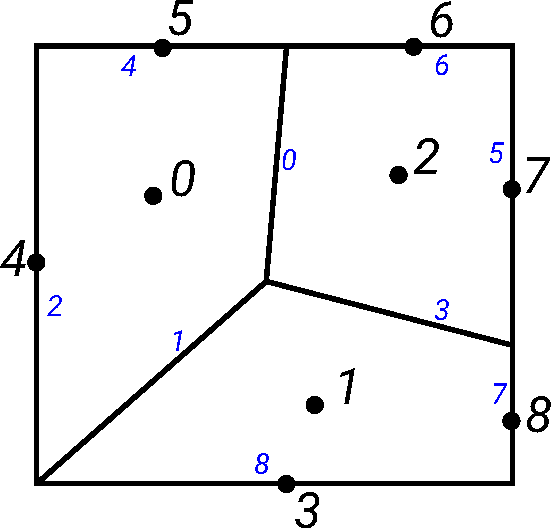
\includegraphics[width=0.25\linewidth]{extended_coll.pdf}
\caption{Расширенный набор точек коллокации}
\label{fig:extended_coll}
\end{figure}

На рис.~\ref{fig:extended_coll}.
представлена конечнообъёмная сетка, содержащая три ячейки
и девять граней. Индексация граней обозначена синими цифрами.
Всего три внутренних грани и шесть граничных.
Согласно стандартной методике конечных
объёмов сеточная функция
будет представлена массивом из трёх элементов.
В расширенном наборе будет девять точек коллокации (обозначены чёрными кругами и проиндексированы чёрными цифрами):
три соответствуют центрам ячеек и ещё шесть -- центрам граничных граней.

Пусть в области с рис.~\ref{fig:extended_coll} нужно решить
уравнение Пуассона \cref{eq:fvm_pois}.
Пусть на ниженей грани задано условие первого рода: $u = C$,
а на правой -- условие третьего рода: $\dsfr{u}{n} = \alpha u + \beta$.

\paragraph{Старый подход}
Согласно ранее рассмотренному методу конечных объёмов
аппроксимация задачи в ячейке с индексом 1 будет иметь следующий вид
$$
\frac{u_1 - u_0}{h_{10}}|\gamma_1|
+\frac{u_1 - u_2}{h_{12}}|\gamma_3|
+\frac{u_1 - C}{h_{13}}|\gamma_8|
+\frac{\alpha u_1 + \beta}{1 - \alpha h_{18}}|\gamma_7|
= V_1 f_1.
$$
Общая размерность матрицы СЛАУ при таком подходе будет
равна $3\times3$, а её элементы в 1-ой строке равны
$$
a_{10} = -\frac{|\gamma_1|}{h_{10}},  \quad
a_{12} = -\frac{|\gamma_3|}{h_{12}},  \quad
a_{11} = \frac{|\gamma_1|}{h_{10}}  + \frac{|\gamma_3|}{h_{12}} + \frac{|\gamma_8|}{h_{13}} + \frac{\alpha|\gamma_7|}{1 - \alpha h_{18}}.
$$
Справа в 1-ой строке будет стоять
$$
b_1 = V_1 f_1 + \frac{C |\gamma_8|}{h_{13}} - \frac{\beta |\gamma_7|}{1 - \alpha h_{18}}.
$$

\paragraph{Новый подход}
В расширенным набором точек коллокаций
матрица правой части будет иметь размерность $9\times9$.
Из них первые три будут собираться согласно классической процедуре
метода конечных объёмов, но учитывая наличие дополнитиельных точек коллокации в центрах
граничных граней. Так, 1-ое уравнение итоговой СЛАУ примет вид
$$
\frac{u_1 - u_0}{h_{10}}|\gamma_1|
+\frac{u_1 - u_2}{h_{12}}|\gamma_3|
+\frac{u_1 - u_3}{h_{13}}|\gamma_8|
+\frac{u_1 - u_8}{h_{18}}|\gamma_7|
= V_1 f_1.
$$
Остальные шесть уравнений будут представлять из себя
аппроксимацию граничных условий для соответствующих граней.
Так, 3-е уравнение будет соответствовать условию первого рода на грани $\gamma_8$:
$$
u_3 = C,
$$
а уравнение 8 -- условию третьего рода на грани $\gamma_7$:
$$
\frac{u_8 - u_1}{h_{18}} = \alpha u_8 + \beta
$$
Переводя рассмотренные уравнения в матричные коэффициенты, получим
следующие ненулевые коээфиициенты итоговой матрицы $\{a_{ij}\}$ и вектора правой части $\{b_i\}$. Для 1-ой строки
$$
a_{10} = -\frac{|\gamma_1|}{h_{10}},  \quad
a_{12} = -\frac{|\gamma_3|}{h_{12}},  \quad
a_{13} = -\frac{|\gamma_8|}{h_{13}},  \quad
a_{18} = -\frac{|\gamma_7|}{h_{18}},  \quad
a_{11} = -(a_{10} + a_{12} + a_{13} + a_{18}), \quad
b_1 = V_1 f_1,
$$
для 3-ей строки
$$
a_{33} = 1, \quad b_3 = C,
$$
для 8-ой строки
$$
a_{81} = -\frac{1}{h_{18}},  \quad
a_{88} = -a_{81} - \alpha, \quad
b_8  = \beta
$$

\subsection{Задание для самостоятельной работы}
\begin{enumerate}
\item
Решить задачу из п.~\ref{sec:hw_fvm2d}, 
с истинными граничными условиями первого рода,
и с граничными условиями первого рода, поставленными
через условия третьего рода.
\item
Убедится, что полученный ответ
с точностью то ошибки решения СЛАУ ($10^{-8}$)
совпадает с результатами, полученным
в двух предыдущих заданиях.
\item
Для постановки с условиями третьего рода
построить график максимального
отклонения граничного значения
полученного сеточной функции $\gvec{u}$ от точного решения в зависимости от выбранного $\eps^{-1}$ из \cref{eq:fvm_bc3_universal}
от точного решения:
$$
n_b = \max_{j > N_c} |u_j - u^e(\vec x_j)|,
$$
$N_c$ -- количество ячеек сетки, $j$ -- индекс граничных точек коллокации, $x_j$ -- координата точки коллокации.

\end{enumerate}

\paragraph{Рекомендации к программированию}
\begin{itemize}
\item
В структуру \cvar{DirichletFaces} необходимо добавить
поле \cvar{icol} -- индекс точки коллокации для текущей грани.
Нумерацию граничных точек коллокации нужно вести
начиная от \cvar{grid.n_cells()} согласно
порядку вектора \cvar{_dirichlet_faces}.
\item
Следует учитывать, что вектор неизвестных \cvar{_u} 
будет иметь длину, большую чем количество ячеек.
В частности, это может привести к ошибке сохранения в vtk.
Чтобы ограничить количество сохраняемых элементов вектора,
вызов сохранения необходимо осуществять с дополнительным параметром:
\begin{cppcode}
	VtkUtils::add_cell_data(_u, "numerical", filename, _grid.n_cells());
\end{cppcode}

\end{itemize}
